\usepackage{tcolorbox}
\usepackage{graphicx}
\usepackage{xcolor}
\tcbuselibrary{skins,breakable}

% ── Title page styling ──────────────────────────────────────────────
\usepackage{tikz}
\renewcommand{\maketitle}{%
  \begin{titlepage}
    \centering
    \vspace*{1cm}
    {\Huge\bfseries Declarative Modeling\\[0.3em] with CP-SAT\par}
    \vspace{0.8cm}
    {\Large\itshape Managing the Complexity of Optimization Modeling\par}
    \vspace{1.2cm}
    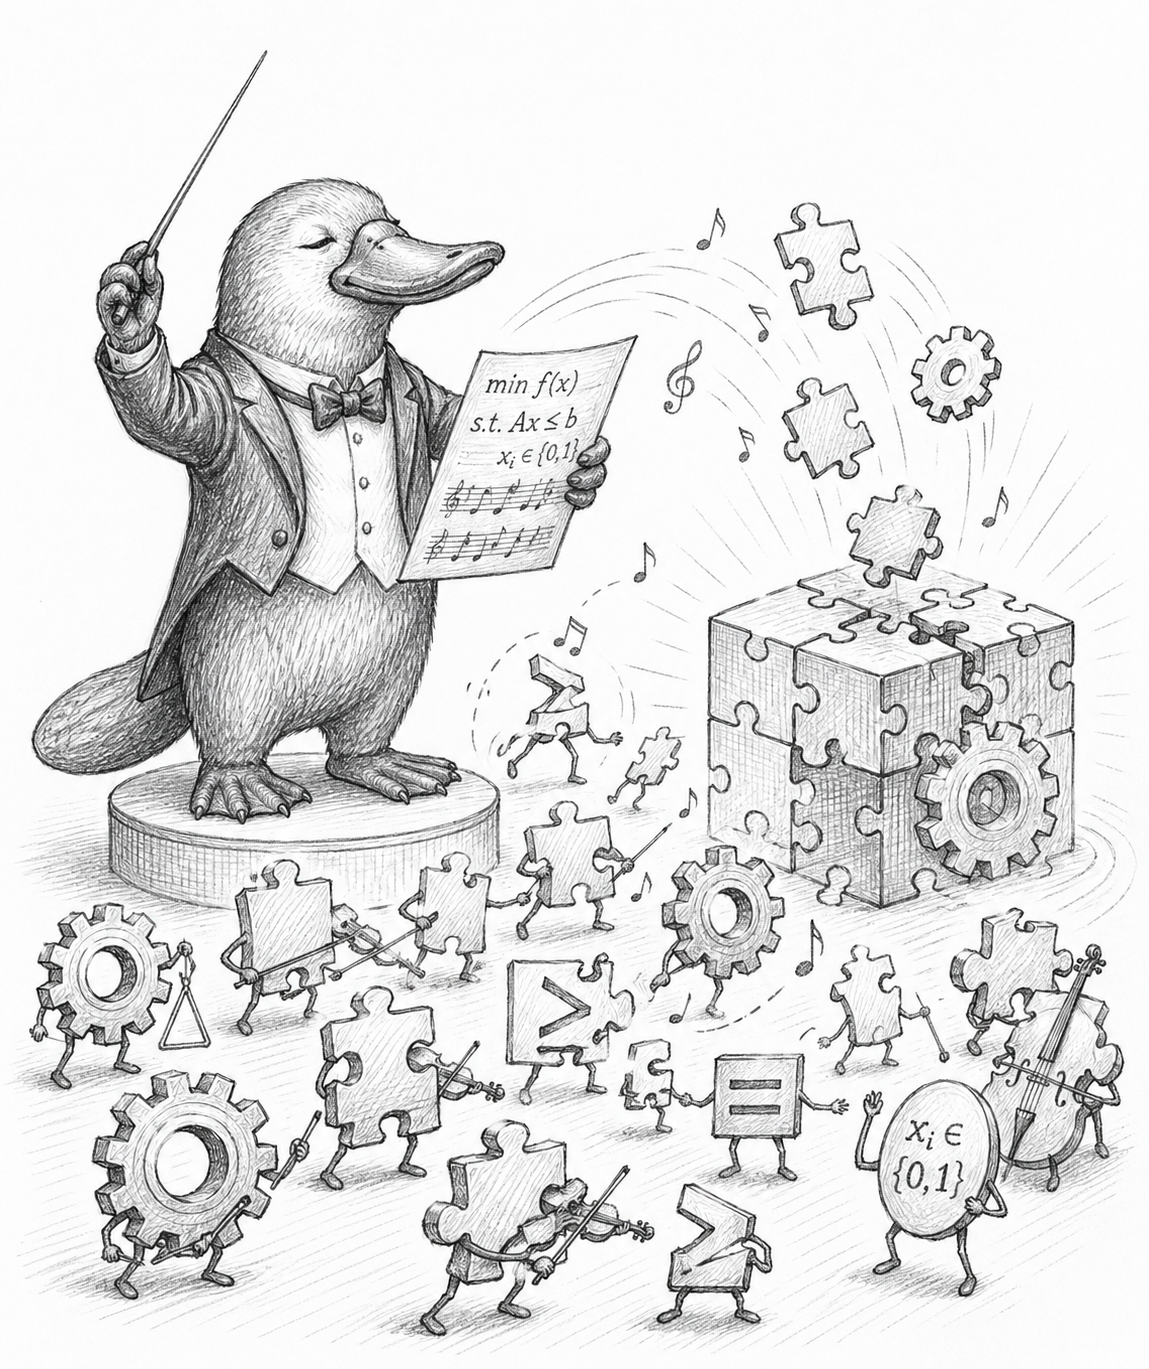
\includegraphics[width=0.55\textwidth]{cover.png}
    \vfill
    {\large Dominik Krupke\par}
    \vspace{0.3em}
    {\normalsize Algorithms Division, TU Braunschweig\par}
    \vspace{0.2em}
    {\small\href{mailto:krupked@gmail.com}{krupked@gmail.com}\par}
    \vspace{1.2em}
    {\footnotesize
      \raisebox{-0.35em}{\doclicenseImage[imagewidth=3em]}\quad
      \textcopyright\ Dominik Krupke. Licensed under
      \href{https://creativecommons.org/licenses/by/4.0/}{CC~BY~4.0}.\par}
    \vspace{0.4em}
    {\footnotesize\href{https://github.com/d-krupke/cpsat-primer}{github.com/d-krupke/cpsat-primer}\par}
  \end{titlepage}
}

% Path to platypus icon assets
\newcommand{\platypusassets}{.assets}

% ── Platypus callouts ────────────────────────────────────────────────
%
% Design: thick colored left rule, pale tinted background, no other
% borders. Platypus icon sits in the top-left margin; the title is set
% inline as the first paragraph of the body, in the accent color.
%
% Usage:
%   \begin{platypusinfo}     ... \end{platypusinfo}      % default title
%   \begin{platypusinfo}[Aside] ... \end{platypusinfo}   % custom title
%
% Variants: platypusinfo (blue), platypustip (green),
%           platypuswarning (amber), platypusbook (violet).

% Width allotted to the icon column (and reserved on the left of the body).
\newlength{\platypusiconwidth}
\setlength{\platypusiconwidth}{42pt}
\newlength{\platypusiconsep}
\setlength{\platypusiconsep}{12pt}

% Title style for the heading at the top of each box's body column.
\newcommand{\platypustitle}[2]{%
  {\bfseries\sffamily\large\color{#1!55!black}#2}\par\vspace{2pt}%
}

% Shared base. Argument 1 = accent color, 2 = icon basename, 3 = title text.
%
% Layout: the upper content is split into two top-aligned minipages —
% icon on the left, title+body on the right. Both columns participate in
% the box's natural height, so the frame always extends at least as far as
% the (potentially tall) platypus icon. Trade-off: minipage-based boxes
% cannot break across pages.
\tcbset{
  platypusbase/.style n args={3}{%
    enhanced,
    sharp corners,
    boxrule=0pt,
    leftrule=3pt,
    colback=#1!4,
    colframe=#1!55!black,
    left=12pt,
    right=12pt,
    top=12pt,
    bottom=12pt,
    fontupper=\normalsize,
    before upper={%
      \begin{minipage}[t]{\platypusiconwidth}%
        \vspace{0pt}% align minipage by its top, not first-line baseline
        \includegraphics[width=\platypusiconwidth,keepaspectratio]%
          {\platypusassets/platypus_#2}%
      \end{minipage}%
      \hspace{\platypusiconsep}%
      \begin{minipage}[t]{\dimexpr\linewidth-\platypusiconwidth-\platypusiconsep\relax}%
        \vspace{0pt}%
        \platypustitle{#1}{#3}%
    },
    after upper={\end{minipage}}%
  }
}

\newtcolorbox{platypusinfo}[1][Note]{%
  platypusbase={blue}{info}{#1}%
}

\newtcolorbox{platypustip}[1][Tip]{%
  platypusbase={green!60!black}{tip}{#1}%
}

\newtcolorbox{platypuswarning}[1][Warning]{%
  platypusbase={orange!85!black}{warning}{#1}%
}

\newtcolorbox{platypusbook}[1][Background]{%
  platypusbase={violet}{book}{#1}%
}
